\documentclass[border=3pt]{standalone}
% Preâmbulo compartilhado pelos diagramas TikZ da aula 5 de IHC (Processos de Design)
\usepackage[T1]{fontenc}
\usepackage[utf8]{inputenc}
\usepackage{lmodern}
\usepackage{amsmath}
\usepackage{xcolor}
\usepackage{tikz}
\usetikzlibrary{arrows.meta,angles,quotes,decorations.pathmorphing,calc,
                positioning,shapes.geometric,shapes.misc,backgrounds,fit,
                math}

% Paleta (mesma dos SVGs originais)
% Paleta da disciplina de IHC: acento roxo (#755099), da capa do livro.
% (o nome "dblue" é mantido para não alterar todos os diagramas)
\definecolor{dblue}{HTML}{755099}
\definecolor{dorange}{HTML}{B3541E}
\definecolor{dgreen}{HTML}{4A7C59}
\definecolor{dred}{HTML}{9C4B4B}
\definecolor{dcream}{HTML}{F4F1EA}
\definecolor{dshade}{HTML}{DDD7C9}

% Função gaussiana (não normalizada por padrão de escala visual)
\pgfmathdeclarefunction{gauss}{3}{%
  \pgfmathparse{1/(#3*sqrt(2*pi))*exp(-((#1-#2)^2)/(2*#3^2))}%
}

% Estilos comuns (prefixo d... para não colidir com chaves internas do pgf)
\tikzset{
  >={Stealth[length=2mm]},
  dguide/.style={gray!55, dashed, line width=0.4pt},
  daxis/.style={gray!60, line width=0.7pt, ->},
  dbody/.style={fill=black!3, draw=black!80, line width=1pt},
  dacc/.style={draw=dblue, line width=1pt},
  dlbl/.style={black!55, font=\small},
  dsub/.style={black!45, font=\footnotesize},
  dstate/.style={circle, draw=black!80, fill=dcream, line width=1pt,
                 minimum size=17mm, font=\large, inner sep=1pt},
  dobs/.style={circle, draw=black!80, fill=dshade, line width=1pt,
               minimum size=14mm, font=\large, inner sep=1pt},
  dbox/.style={rounded corners=2pt, draw=black!80, fill=dcream, line width=1pt,
               align=center, inner sep=6pt},
  dop/.style={circle, draw=black!80, fill=white, line width=1pt,
              minimum size=6mm, inner sep=0pt, font=\small},
  dtrans/.style={->, dblue, line width=1pt},
  dmeas/.style={->, dorange, line width=1pt},
  dcurve/.style={line width=1pt, dblue},
  dcurveb/.style={line width=1.4pt, dorange},
}

\begin{document}
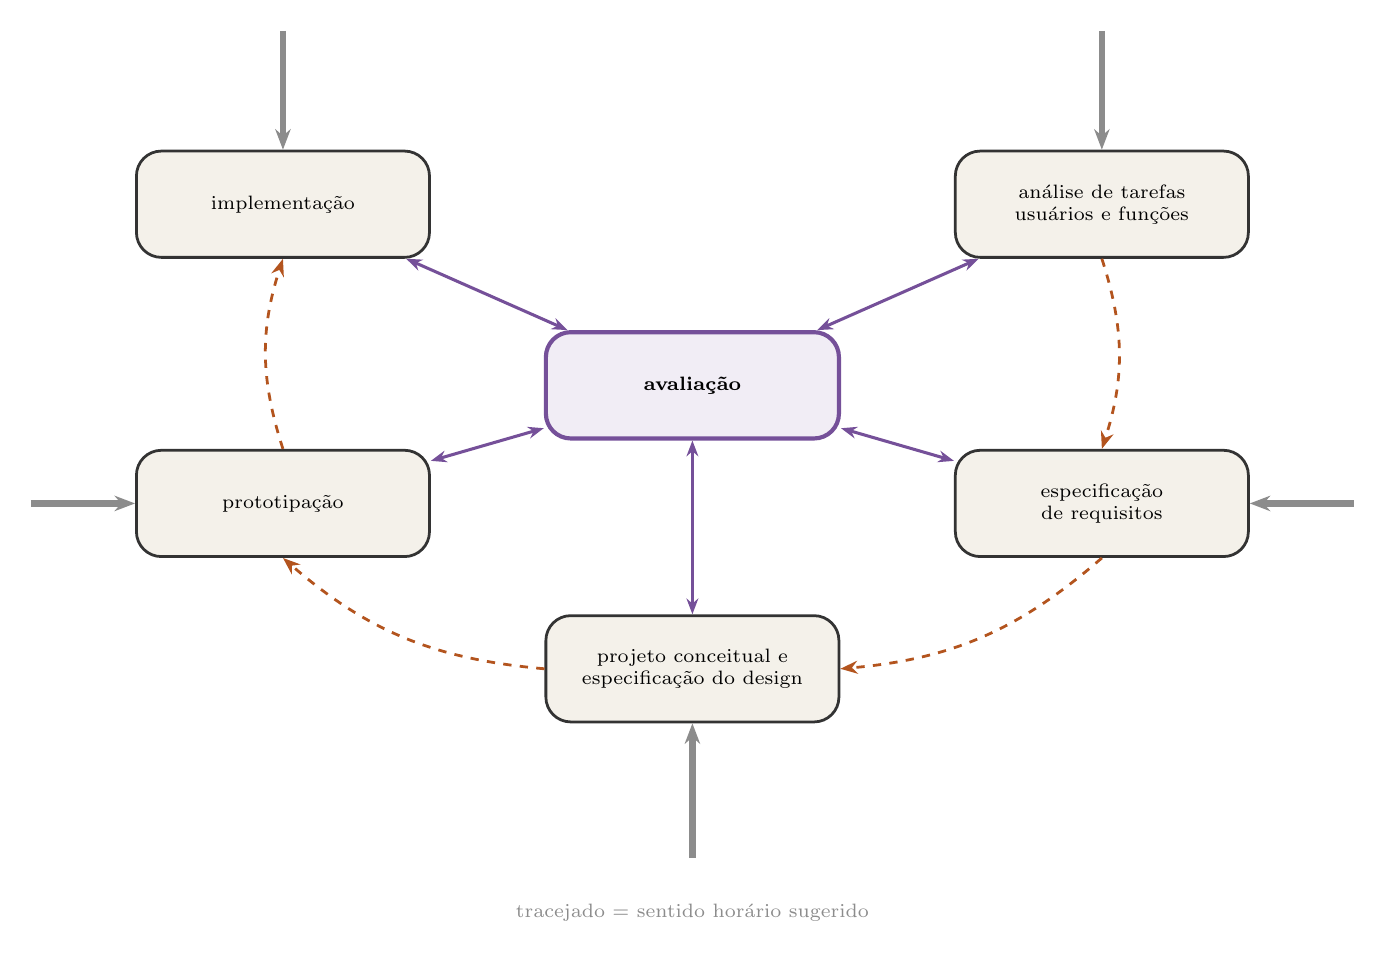
\begin{tikzpicture}[x=1cm,y=1cm,
   act/.style={dbox, rounded corners=9pt, text width=3.3cm, minimum height=1.35cm, font=\scriptsize}]

  \node[act, draw=dblue, line width=1.5pt, fill=dblue!10] (av) at (0,0) {\textbf{avaliação}};

  \node[act] (at) at (5.2,2.3) {análise de tarefas\\usuários e funções};
  \node[act] (er) at (5.2,-1.5) {especificação\\de requisitos};
  \node[act] (pc) at (0,-3.6) {projeto conceitual e especificação do design};
  \node[act] (pr) at (-5.2,-1.5) {prototipação};
  \node[act] (im) at (-5.2,2.3) {implementação};

  \foreach \n in {at,er,pc,pr,im} { \draw[<->, dblue, line width=1.1pt] (av) -- (\n); }

  % sentido horário (sugestão)
  \draw[dmeas, dashed, -{Stealth[length=2.2mm]}, bend left=18] (at.south) to (er.north);
  \draw[dmeas, dashed, -{Stealth[length=2.2mm]}, bend left=18] (er.south) to (pc.east);
  \draw[dmeas, dashed, -{Stealth[length=2.2mm]}, bend left=18] (pc.west) to (pr.south);
  \draw[dmeas, dashed, -{Stealth[length=2.2mm]}, bend left=18] (pr.north) to (im.south);

  % entradas possíveis
  \foreach \n in {at,pc,pr} {}
  \draw[-{Stealth[length=2.6mm]}, black!45, line width=2.4pt] (5.2,4.5) -- (at.north);
  \draw[-{Stealth[length=2.6mm]}, black!45, line width=2.4pt] (-5.2,4.5) -- (im.north);
  \draw[-{Stealth[length=2.6mm]}, black!45, line width=2.4pt] (0,-6.0) -- (pc.south);
  \draw[-{Stealth[length=2.6mm]}, black!45, line width=2.4pt] (-8.4,-1.5) -- (pr.west);
  \draw[-{Stealth[length=2.6mm]}, black!45, line width=2.4pt] (8.4,-1.5) -- (er.east);

  \node[dsub, font=\scriptsize, align=center, text width=11cm] at (0,-6.7) {tracejado = sentido horário sugerido};

\end{tikzpicture}
\end{document}
